\begin{figure}[H]
  \centering
  \textbf{Varying states }
  \newline
  \newline
  \pgfplotsset{
    scale only axis,
    legend style={at={(0,0.8)}, anchor=west, font=\tiny},
    xmin=7,
  }
  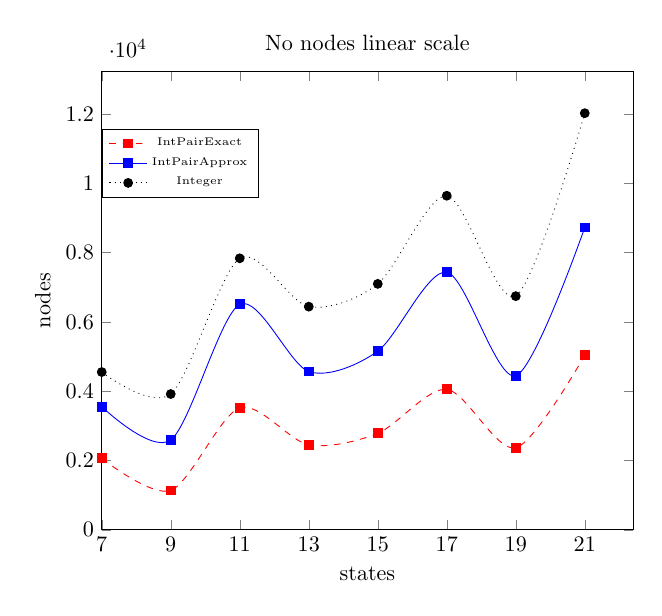
\begin{tikzpicture} [scale=0.8]
    \begin{axis}[
        title=No nodes linear scale,
        ylabel=nodes,
        xtick=data,
        ymin=0, 
        xlabel=states ]
      \addplot[smooth,mark=square*, mark options={solid},red, dashed]
      coordinates{ (7, 2062) (9, 1136) (11, 3521) (13, 2452) (15, 2784) (17, 4053) (19, 2365) (21, 5039)
      }; \label{ie_plot} \addlegendentry{IntPairExact}
      \addplot[smooth,mark=square*, mark options={solid},blue]
      coordinates{ (7, 3553) (9, 2592) (11, 6505) (13, 4568) (15, 5156) (17, 7433) (19, 4444) (21, 8725)
      }; \label{ia_plot} \addlegendentry{IntPairApprox}
      \addplot[smooth,mark=*,mark options={solid},black, dotted]
      coordinates{ (7, 4552) (9, 3918) (11, 7834) (13, 6439) (15, 7096) (17, 9639) (19, 6742) (21, 12021)
      }; \label{int_plot} \addlegendentry{Integer}
    \end{axis}
  \end{tikzpicture}
  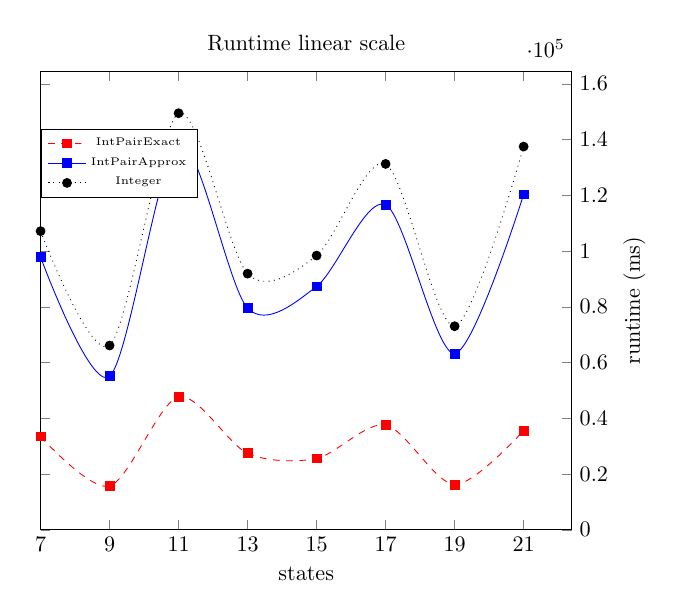
\begin{tikzpicture} [scale=0.8]
    \begin{axis}[
        yticklabel pos=right,
        xtick=data,
        title=Runtime linear scale,
        ylabel=runtime (ms),
        xlabel=states,
        ymin=0, ]
      \addplot[smooth,mark=square*,mark options={solid},red, dashed]
      coordinates{ (7,33465) (9,15686) (11,47674) (13,27424) (15,25602) (17,37602) (19,16206) (21,35578)
      }; \label{IntPairExact Run}
      \addplot[smooth,mark=square*,mark options={solid},blue]
      coordinates{ (7,97813) (9,55060) (11,138726) (13,79518) (15,87294) (17,116620) (19,63208) (21,120264)
      }; \label{IntPairApprox Run}
      \addplot[smooth,mark=*,mark options={solid},black, dotted]
      coordinates{ (7,107122) (9,66098) (11,149430) (13,91884) (15,98370) (17,131234) (19,73028) (21,137458)
      }; \label{IntegerRun}
      \addlegendentry{IntPairExact}
      \addlegendentry{IntPairApprox}
      \addlegendentry{Integer}
    \end{axis}
  \end{tikzpicture}

  
\begin{tikzpicture}[scale=1.4]
    \draw[very thick] (-4,0) -- (4,0);
    \draw[draw=white] (-5,-0.2) -- (5,-0.2);
  \end{tikzpicture}


  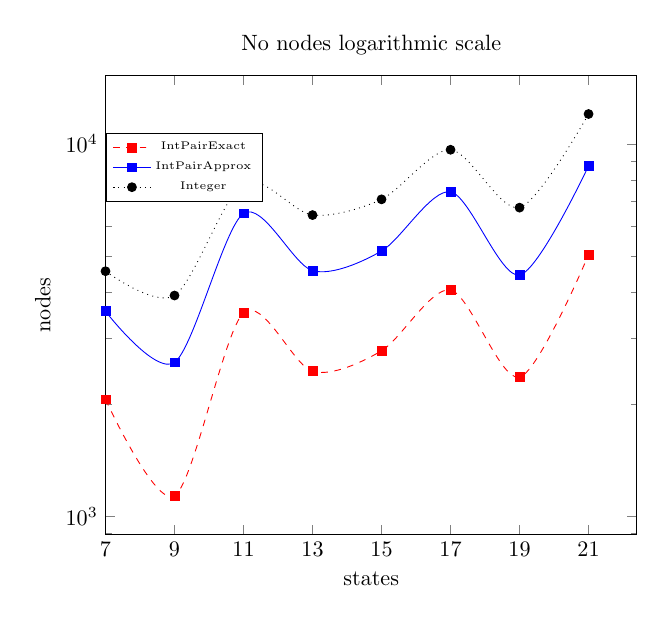
\begin{tikzpicture} [scale=0.8]
    \begin{semilogyaxis}[
        title=No nodes logarithmic scale,
        ylabel=nodes,
        xtick=data,
        ymin=0, 
        xlabel=states ]
     \addplot[smooth,mark=square*, mark options={solid},red, dashed]
      coordinates{ (7, 2062) (9, 1136) (11, 3521) (13, 2452) (15, 2784) (17, 4053) (19, 2365) (21, 5039)
      }; \label{ie_plot} \addlegendentry{IntPairExact}
      \addplot[smooth,mark=square*, mark options={solid},blue]
      coordinates{ (7, 3553) (9, 2592) (11, 6505) (13, 4568) (15, 5156) (17, 7433) (19, 4444) (21, 8725)
      }; \label{ia_plot} \addlegendentry{IntPairApprox}
      \addplot[smooth,mark=*,mark options={solid},black, dotted]
      coordinates{ (7, 4552) (9, 3918) (11, 7834) (13, 6439) (15, 7096) (17, 9639) (19, 6742) (21, 12021)
      }; \label{int_plot} \addlegendentry{Integer}

    \end{semilogyaxis}
  \end{tikzpicture}
  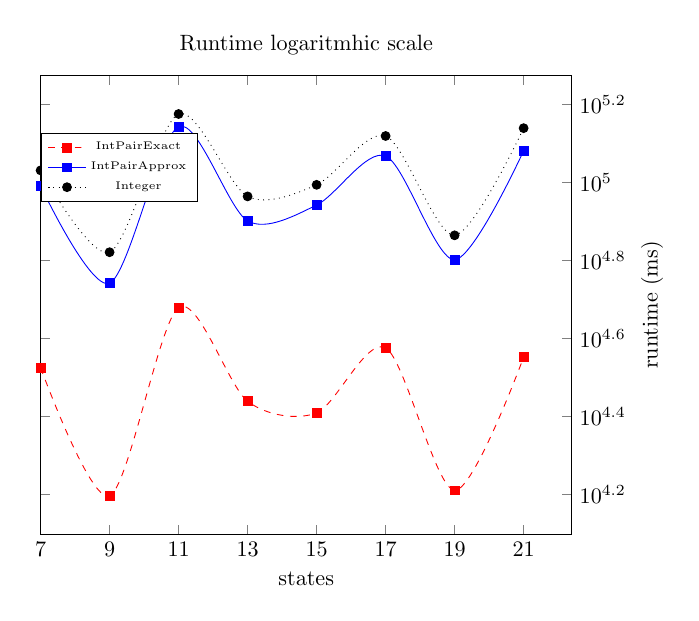
\begin{tikzpicture} [scale=0.8]
    \begin{semilogyaxis}[
        title=Runtime logaritmhic scale,
        yticklabel pos=right,
        xtick=data,
        ylabel=runtime (ms),
        xlabel=states,
        ymin=0,  ]
      \addplot[smooth,mark=square*,mark options={solid},red, dashed]
      coordinates{ (7,33465) (9,15686) (11,47674) (13,27424) (15,25602) (17,37602) (19,16206) (21,35578)
      }; \label{IntPairExact Run}
      \addplot[smooth,mark=square*,mark options={solid},blue]
      coordinates{ (7,97813) (9,55060) (11,138726) (13,79518) (15,87294) (17,116620) (19,63208) (21,120264)
      }; \label{IntPairApprox Run}
      \addplot[smooth,mark=*,mark options={solid},black, dotted]
      coordinates{ (7,107122) (9,66098) (11,149430) (13,91884) (15,98370) (17,131234) (19,73028) (21,137458)
      }; \label{IntegerRun}
      \addlegendentry{IntPairExact}
      \addlegendentry{IntPairApprox}
      \addlegendentry{Integer}
    \end{semilogyaxis}
  \end{tikzpicture}
  \caption{{Caption}}\label{fig:}
\end{figure}
